\begin{figure}[bp]
    \centering
    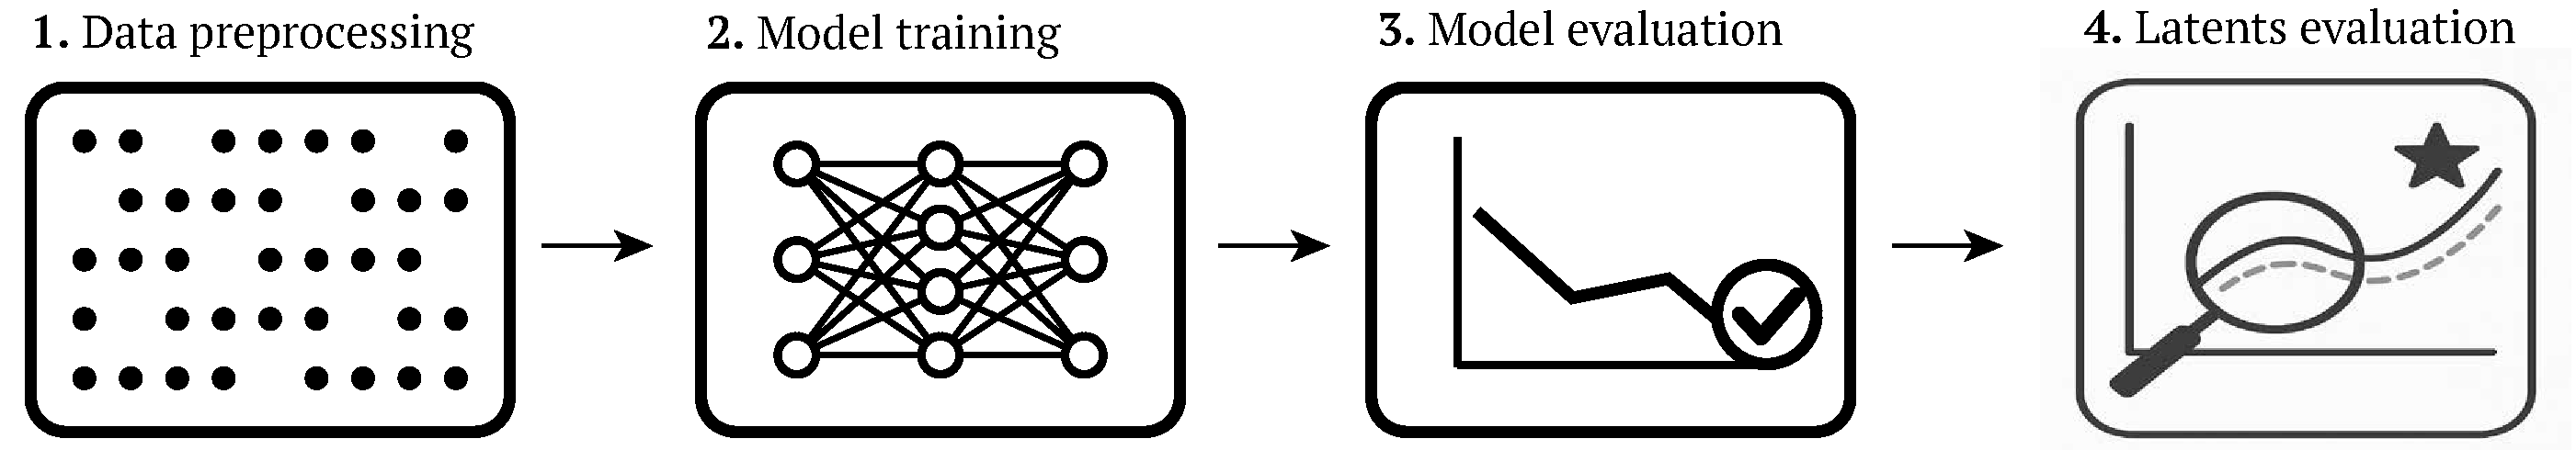
\includegraphics[width=\linewidth]{figures/nldisco_pipeline.pdf}
    \caption{
        \textbf{The NLDisco pipeline.} \\
        \small The NLDisco pipeline has four stages: 1) Spatiotemporal binning and processing of neural data; 2) Training a model; 3) Evaluating the model; 4) Evaluating the model's latents for feature interpretability. Steps 1-3 can be either semi- or fully-automated.
        \vspace{-1em}
    }
    \label{figure:nldisco_pipeline}
\end{figure}

\newcommand{\sedarchcaption}{
\textbf{Model architecture} \\
\small
(\textbf{a}) Natural, ``real-world'' features $x$ are encoded by neural activity $y$. In this example, three active (of six total) features are simultaneously represented by the joint activity of three neurons.
(\textbf{b}) An SED reconstructs target neural activity $\psi$ as $\hat{\psi}$ from input $y$ through sparsely active latents $z$. When training is successful, the learned latents $z$ correspond to natural features $x$. Reconstructing the input population itself ($\psi = y$) gives an autoencoder; reconstructing a separate but related target population gives a transcoder. By default, one training example is a single timebin.
(\textbf{c}) A Matryoshka SED divides the latents into nested levels $L_1 \subset L_2 \subset L_3$, each of which attempts a full reconstruction of $\psi$. Black dashed boxes mark the latents included at a given level and orange dashed boxes mark latents added at higher levels. Here, batch top-$k$ selects one additional active latent at each level (yellow), allowing lower (higher) levels to capture coarser (finer) features.
(\textbf{d}) A W-SED instead treats a sequence of $S$ timebins of $N$ recorded units, $\mathbf{Y}\in\mathbb{R}^{S\times N}$, as one training example and reconstructs all $S$ bins of a target $\mathbf{\Psi}\in\mathbb{R}^{S\times N}$ as $\hat{\mathbf{\Psi}}$ (the batch dimension is omitted throughout). A FW-SED encoder linearly projects the vectorized window to the $D$ latents $\mathbf{z}$; alternatively, a TW-SED encoder treats each timebin's population state as a token, integrates temporal context via self-attention, and projects the temporally contextualized final token to the latents. The latents pass through ReLU and batch top-$k$ (optionally with Matryoshka levels), and each active latent contributes a timebin-by-unit activity pattern to the full reconstruction $\hat{\mathbf{\Psi}}$. The loss is a weighted average of per-timebin losses, $\sum_s w_s \ell_s / \sum_s w_s$; reconstruction quality is also reported per timebin. An optional shift-equivariant mode (each latent is a motif that may occur at any timebin) is described in \hyperref[subsubsection:model_architecture_training]{\ref*{subsubsection:model_architecture_training}}.
}
\begin{figure}[bp]
    
\includegraphics[width=\linewidth]{figures/sed_arch.pdf}
    \caption{
        \sedarchcaption
        \vspace{-1em}
    }
    \label{figure:sed_arch}
\end{figure}

\section{Methods: The NLDisco pipeline}
\label{section:methods}

The NLDisco pipeline transforms high-dimensional neural data into a set of interpretable latents in four stages (\autoref{figure:nldisco_pipeline}), the first three of which can be fully automated.

\vspace{-0.5em}
\paragraph{Stage 1: Data preprocessing.}

The first stage prepares neural data into a $\text{timebin} \times \text{unit}$ matrix for model training. NLDisco has utilities to work directly with outputs from common spike sorters such as Kilosort~\citep{pachitariu_2016_kilosort}, and can aggregate spikes into timebins for each recorded unit and normalize the resulting activity. Users may also provide their own preprocessed $\text{timebin} \times \text{unit}$ data, for example two-photon calcium-imaging regions of interest extracted by Suite2p~\citep{pachitariu_2017_suite2p}.

\vspace{-0.5em}
\paragraph{Stage 2: Model training.}

In the second stage, an SED with configurable dictionary width $D$ is trained to reconstruct target neural activity. Training is unsupervised and uses only neural activity; behavioral and environmental labels enter only post hoc, for latent interpretation and evaluation. The goal is for the model's hidden layer neurons (latents) to capture disentangled, interpretable representations encoded by the population activity (\autoref{figure:sed_arch}a). Sparsity encourages a monosemantic dictionary in which each latent corresponds to a single feature: for example, a latent learned from visual cortical activity may represent a property of a visual stimulus, while one learned from motor cortical activity may represent an aspect of movement. Each active latent contributes to the target reconstruction through explicit decoder weights, and its encoder weights link its activation to constituent source neural activity.

The SED configuration can be selected according to the scientific question and temporal structure of the data (\autoref{figure:sed_arch}b,c,d). A vanilla SED treats each timebin independently. A W-SED treats a sequence $\mathbf{Y}\in\mathbb{R}^{S\times N}$ of $S > 1$ timebins and $N$ recorded units as one example, allowing each latent to represent a timebin-by-unit pattern. W-SEDs have two encoder variants: the Flat-window encoder (FW-SED) linearly projects the vectorized window, while the Transformer-window encoder (TW-SED) integrates timebin tokens using self-attention. Both reconstruct the complete window through a sparse latent code; the TW-SED additionally supports an optional shift-equivariant mode to capture motifs that may occur at different positions within a window across examples. Nested Matryoshka levels~\citep{bussmann_2025_msae} can be used with either the vanilla or W-SED: each nested level attempts to reconstruct the full target using a progressively larger subset of the shared latent dictionary, encouraging multi-scale representations and mitigating feature absorption, in which a specific feature partially subsumes a more general one~\citep{chanin_2024_feature_absorption}. For example, separate Matryoshka SED latents can recover both an encompassing place field and a narrower field nested within it, without the narrower-field latent hiding the activity associated with the broader field (see \hyperref[subsection:synthetic_results]{\ref*{subsection:synthetic_results}}).

Independently of the architectural choice, an SED can be trained as an autoencoder~\citep{cunningham_2023_saes} that reconstructs its input population, or as a transcoder~\citep{dunefsky_2024_transcoders} that reconstructs one neural population based on another, potentially across brain regions, recording sessions, or subjects. These configurations support analysis of both the intrinsic representational structure of a population and how representations are transformed across regions, sessions, or subjects. All configurations use batch top-$k$ sparsification, a batch-level variant of TopK~\citep{gao_2025_topk_saes} that preserves the $Bk$ largest latent activations across a batch of size $B$~\citep{bussmann_2024_batchtopk}. Unlike indirect approaches such as an L1 penalty, batch top-$k$ directly controls total sparsity while allowing individual examples to recruit different numbers of latents.

NLDisco also supports automated hyperparameter sweeps of architectural and training optimization configurations across CPUs or GPUs. The complete training procedure and hyperparameter guidance are described in \hyperref[subsubsection:model_architecture_training]{\ref*{subsubsection:model_architecture_training}}.

\paragraph{Stage 3: Model evaluation.}

Following training, model quality is evaluated using a suite of quantitative metrics. NLDisco adapts domain-general metrics from SAEBench~\citep{karvonen_2025_saebench} and adds metrics tailored to neural data. Although these metrics do not directly establish latent interpretability, they test whether the model has learned a sparse, accurate, and robust representation suitable for subsequent inspection.

Reconstruction fidelity is measured using variance explained (\metric{R^2}) and reconstruction-to-target cosine similarity across both units and examples (\autoref{figure:model_eval}, bottom). For W-SEDs, reconstruction quality is additionally reported for each timebin in the window. Evaluation distinguishes dictionary width $D$ from activation sparsity $k$. Increasing either can improve reconstruction, but reconstruction alone does not establish interpretability. NLDisco therefore also examines latent \metric{L0} -- the number of active latents per example -- and latent activation density across the dataset (\autoref{figure:model_eval}, top), which together can reveal failure modes such as representational collapse into many persistently active latents, or feature death in which latents never activate. Optional diagnostics include latent ablation importance and spectral comparisons between reconstructed and target activity (\hyperref[subsubsection:model_evaluation_details]{\ref*{subsubsection:model_evaluation_details}}). Raw model parameters, gradients, and activations remain available for bespoke analyses.

\paragraph{Stage 4: Latents evaluation.}

For exploratory discovery, users can survey all active latents or a random subset, inspecting representative activating and inactive episodes alongside behavior. Recurring patterns suggest feature descriptions; counterexamples refine them. Source activity traceback identifies contributing units and timebins, guiding hypotheses for testing on separate recordings or in targeted experiments. Evaluation methods and metrics are detailed in \hyperref[subsubsection:latents_evaluation_details]{\ref*{subsubsection:latents_evaluation_details}} and demonstrated in \nameref{section:results}.
